\documentclass[a4paper]{article}

\usepackage[spanish]{babel}
\usepackage[utf8]{inputenc}
\usepackage[T1]{fontenc}
\usepackage{float}
\usepackage{amsmath,amssymb,amsfonts}
\usepackage{graphicx}
\usepackage{subfig}		
\usepackage{subcaption}
\usepackage{verbatim}					
\usepackage{url}
\usepackage{tikz}
\usetikzlibrary{arrows.meta}
\tikzset{>=Stealth}
\AtBeginDocument{\shorthandoff{<>}}

\usepackage[most]{tcolorbox}
\usepackage{psfrag}		
\usepackage{xcolor}
\usepackage[a4paper,top=1cm,bottom=1.5cm,left=3cm,right=3cm,marginparwidth=2.5cm]{geometry}
\usepackage{palatino}
\usepackage{environ}     % para definir entornos que eliminan su cuerpo
\setlength{\parindent}{5pt} 
\setlength{\parskip}{0.5\baselineskip}




\newif\ifprintanswers
\printanswerstrue

\definecolor{miazul}{RGB}{25,43,191}

% Definición de solution con recuadro
\NewEnviron{solution}{%
  \ifprintanswers
    \begin{tcolorbox}[
      colframe=black,     % color del borde
      colback=white,      % fondo blanco
      boxrule=0.8pt,      % grosor de la línea
      arc=0pt,            % esquinas agudas
      left=4pt,           % espacio interior izquierdo
      right=4pt,          % espacio interior derecho
      top=4pt,            % espacio interior superior
      bottom=4pt,         % espacio interior inferior
      before skip=0.5\baselineskip,
      after skip=0.5\baselineskip
    ]
      \textbf{\textit{Respuesta:}}\quad
      \BODY
    \end{tcolorbox}
  \fi
}

\renewcommand{\thefootnote}{\fnsymbol{footnote}}

\begin{document}

\begin{center}
    \includegraphics[width=1cm]{escudo.jpg}

    \vspace{0.5cm}

    \large \textbf{Finanzas Internacionales}\\\textbf{Ayudantía 1}\footnote{Correo: joamartine@fen.uchile.cl}
\end{center}

\section{Cuentas del Comercio Exterior}

\subsection{Comentes}

Se puede medir el producto de una economía cerrada como el gasto total de la economía, el cual se compondría de tres componentes que conforman la demanda interna: $$Y = \underbrace{C+I+G}_{A}.$$ La cual abrirse al comercio exterior suma una componente más, las exportaciones netas $XN$. La diferencia entre exportaciones e importaciones se define como balanza comercial, el saldo de la balanza comercial se define: $$XN = X-M$$

\begin{itemize}
    \item[a)] Explique en sus propias palabras lo que implica una desigualdad entre el gasto interno y el producto de una economía abierta. ¿En qué caso tendríamos un déficit o un superávit?
    \begin{solution}
        La balanza comercial $XN$ captura la diferencia entre lo que el país produce y lo que gasta internamente (absorción). Si $XN > 0$, entonces $Y > A$, lo que implica que el país está produciendo más de lo que absorbe. Por el contrario si $XN < 0$ denota una economía que está gastando más de lo que produce, por lo que en el neto se está cubriendo esta demanda por importaciones.

        $$Y = A+XN$$

        Si en el neto se recurre a importaciones para cubrir la demanda se muestra como una balanza deficitaria, mientras que si el gasto interno no supera lo producido por la economía implica exportaciones que dejan un superávit en la balanza.
    \end{solution}
    \item[b)] Según los resultados de la balanza de pagos de 2024, en Chile hubo un alza en la demanda del cobre, una reducción de los envíos de productos químicos además de un aumento generalizado por vestuario y calzado, celulares y alimentos de otros países. Explique como cada una de estas cosas influenciarían en la balanza comercial.
\begin{solution}
\begin{itemize}
    \item Un aumento en la demanda de cobre a nivel mundial aumenta las exportaciones y el saldo de la balanza comercial. 
    \item Una reducción de los envíos de productos químicos (derivados del litio por ejemplo) reducen las exportaciones y con ello el saldo de balanza comercial. 
    \item Un aumento por la demanda de bienes de consumo de otros países incrementa las importaciones y con ello reducen la balanza comercial.
\end{itemize}
\end{solution}
\item[c)] El siguiente gráfico muestra la cuenta corriente de Chile entre 1990 y 2023. Explique por qué la cuenta corriente mejoró durante el boom del cobre de mediados de los 2000 y luego se deterioró, relacionando su respuesta con el concepto de balance estructural y la visión de persistencia del shock.
\begin{center}
        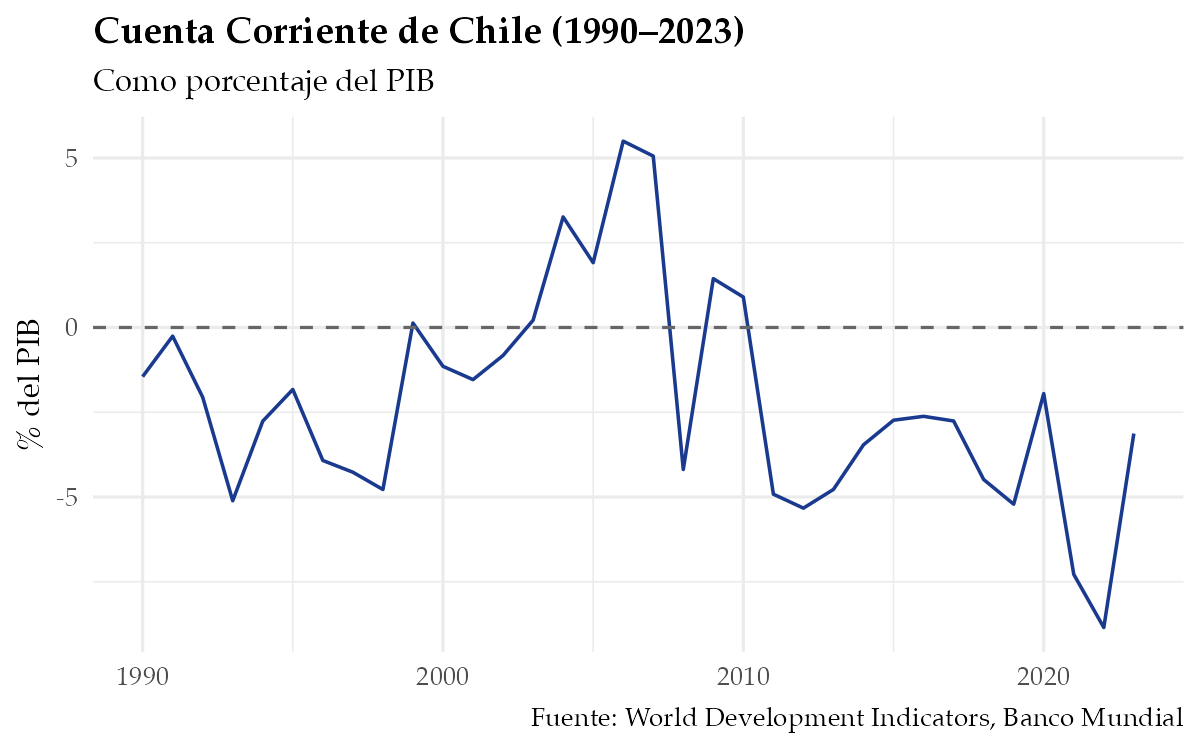
\includegraphics[width=10cm]{cc_rcode/outputs/cc_chile.png}
    \end{center}
\begin{solution}
    

    Durante el boom del precio del cobre (2004--2007) la cuenta corriente de Chile mejoró notablemente, llegando a un superávit cercano al 6\% del PIB en 2007. 

    \begin{itemize}
        \item \textbf{Visión inicial del shock como transitorio.} Al comienzo del boom, los agentes y el gobierno percibieron el alza del cobre como un shock temporal. Bajo esa percepción, la respuesta óptima de una economía pequeña y abierta es ahorrar el ingreso extra en lugar de consumirlo o invertirlo de inmediato. Esto se refleja directamente en un superávit de cuenta corriente: $CC = S_n - I$, con $S_n$ elevado porque el ingreso transitorio se ahorra.

        \item \textbf{Balance estructural y ahorro fiscal.} El gobierno de Chile adoptó explícitamente la regla de balance estructural del cobre: los ingresos fiscales del cobre se evalúan al precio de largo plazo (precio de referencia), y solo ese ingreso estructural financia el gasto. El excedente por sobre el precio de referencia se acumula en el Fondo de Estabilización de los Ingresos del Cobre y posteriormente el Fondo de Estabilización Económica y Social (FEES), lo que equivale a ahorro público que mejora la cuenta corriente.
    \end{itemize}

    Cuando el precio del cobre se mantuvo elevado por varios años, los agentes comenzaron a revisar al alza su percepción de persistencia del shock. Si el ingreso alto es permanente, ya no hay razón para seguir ahorrándolo. Bajo un shock permanente el modelo de suavizamiento del consumo predice $CC \approx 0$, pues el mayor ingreso se consume en vez de ahorrarse. Adicionalmente, el propio auge del cobre estimuló la inversión en el sector minero (aumentando la demanda de bienes de capital importados), lo que redujo el saldo de cuenta corriente. Ambos efectos empujaron la cuenta corriente hacia el déficit durante la segunda mitad del boom y los años posteriores.

    Esto se verifica directamente en el gráfico de ahorro e inversión: durante 2005--2008 el ahorro nacional superó a la inversión, generando el superávit; luego la brecha se invirtió y la inversión minera superó al ahorro, explicando el déficit posterior.

    \begin{center}
        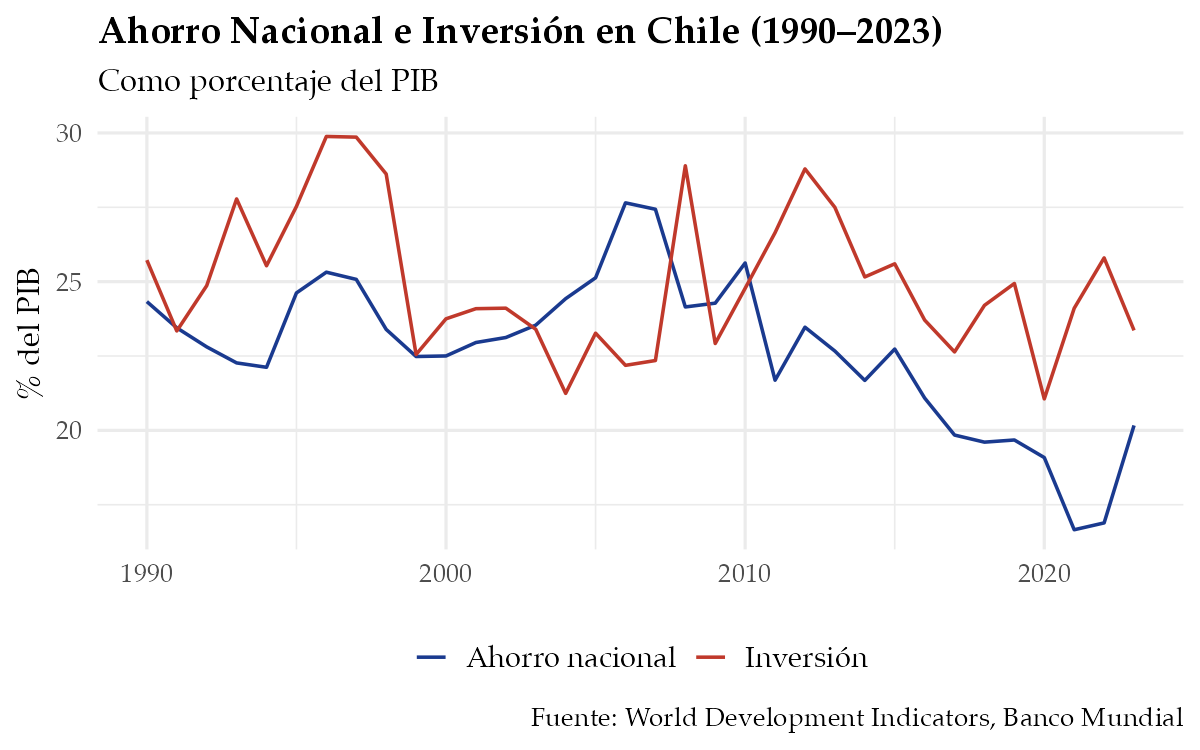
\includegraphics[width=10cm]{cc_rcode/outputs/ahorro_inversion_chile.png}
    \end{center}
\end{solution}
\end{itemize}


Considerando exportaciones, importaciones, impuestos, transferencias del gobierno y pagos de factores al exterior el producto se puede escribir como $$\underbrace{Y -T+TR-F }_{YD}= C+I+G-T+TR+XN-F$$ $$YD = C+I+G-T+TR+XN-F$$
 
\begin{itemize}
    \item[d)] Escriba en base a lo anterior el ahorro público, privado y externo.
    \begin{solution}
        \begin{align*}
        \underbrace{YD-C}_\text{Ahorro privado} = I+G-T+TR+XN-F \\
        YD-C + \underbrace{T-TR-G}_{\text{Ahorro público}} = I+XN-F \\
        YD-C \underbrace{-XN+F}_{\text{Ahorro Externo}} +T-TR - G = I \\
        \implies S_p+S_e+S_g = I
        \end{align*}
    \end{solution}
    \item[e)] ¿Por qué el ahorro externo equivale a la cuenta corriente? Conceptual y matemáticamente.
    \begin{solution}
        En una economía abierta, si un país gasta más de lo que produce, necesita financiamiento externo: está absorbiendo ahorro del resto del mundo. A ese financiamiento lo llamamos ahorro externo.
        
        Ese desajuste entre gasto e ingreso nacional se refleja en la cuenta corriente (CC) de la balanza de pagos. Si hay déficit en la cuenta corriente, el país necesita ahorro externo; si hay superávit, el país está prestando al resto del mundo (es decir, genera ahorro externo positivo para otros).
        \begin{align*}
            S_e &= I-S_p-S_g \\
            & = I-YD+C - T+TR+G \\
            & = I+C-T+TR+G - (Y-T+TR-F) \\
            & = I+C+G+F-Y \\
            & = F + C+I+G-(C+I+G+XN) \\
            & = F-XN
        \end{align*}
        El ahorro externo son las importaciones que el país le compra menos lo que el país le vende más el pago neto que el país tiene que pagar al exterior.

        Por lo tanto, 
        \begin{itemize}
            \item El déficit en cuenta corriente es equivalente al ahorro externo. 
            \item El déficit de cuenta corriente mide el exceso de gasto sobre ingreso.
        \end{itemize}
        \end{solution}
        \end{itemize}

        Las dos definiciones más utilizadas para el saldo de cuenta corriente son 
        \begin{align*}
            &CC = S_n -I \\
            &CC = X-M-F
        \end{align*}
        \begin{itemize}
        \item[f)] La administración de Donald Trump con tal de reducir el déficit de cuenta corriente deciden imponer aranceles, ¿cuál sería el efecto de los aranceles de la cuenta corriente? Explique por qué se dice que el déficit de cuenta corriente de Estado Unidos ayudó a financiar su exceso d inversión. 

        \begin{solution}
            Los aranceles disminuyen las importaciones y por tanto el saldo de balanza comercial aumenta, con ello también la cuenta corriente.

            Dado un determinado ahorro nacional, a mayor sea la inversión que el país reciba mayor será el déficit de cuenta corriente.
        \end{solution}

        \item[g)] ¿Qué componentes tienen los pagos netos a los factores del exterior? 
        \begin{solution}
            Rentas (renta primaria): registra la entrada y salida de pagos por servicios de factores. Por ejemplo, si una empresa transnacional produce utilidades dentro del país y las usa para generar dividendos a sus accionistas en el exterior, eso es una salida. Ello corresponde al pago que hacemos por usar los servicios del capital en el exterior (ejemplo utilidades del cobre). Los intereses sobre deuda externa también se registran aquí.

            Cabe destacar que las transferencias unilaterales (remesas, donaciones) \textbf{no} forman parte de $F$: son un componente separado de la cuenta corriente, denominado renta secundaria. $F$ incluye únicamente rentas de factores (remuneración de empleados y rentas de la inversión).

        \end{solution}

        \item[h)] ¿Cuáles son las componentes de la balanza de pago? Defina Cuenta Financiera.
        \begin{solution}
            La balanza de pagos registra todas las transacciones que tiene el país con el exterior, por lo que incluye a la cuenta corriente. Además incluirá la cuenta de financiera, que registra todo lo que un país pide prestado y le presta al resto del mundo.

        \end{solution}

        \item[i)] Si una empresa se endeuda con el extranjero para financiar sus inversiones, indique donde se registraría el préstamo, los intereses y la amortización. 

        \begin{solution}
            El préstamo entraría directamente en la cuenta financiera, aumenta el saldo. Sin embargo la amortización de la deuda representa una salida de capital por lo que disminuye el saldo.

            El pago de intereses se registra en la \textbf{cuenta corriente}, dentro del rubro de rentas (renta primaria), pues es el pago por el uso de un factor de producción —el capital— propiedad del exterior. La cuenta financiera solo recoge el principal del préstamo y su amortización.
        \end{solution}
    
    \end{itemize}



\subsection{Matemático I}

 Considere un país que tiene un PIB de 100 mil millones de pesos y un gasto agregado (A) de 103 mil millones de pesos. El país tiene una deuda externa (es su única relación financiera con el resto del mundo) de 10 mil millones de dólares. Si el tipo de cambio de este país es de 2 pesos por dólar y la tasa de interés internacional (que
se paga por la deuda externa) es de 5\%, calcule:

\begin{enumerate}

    \item[a)] Calcule el PNB (Producto Nacional Bruto).
    \begin{solution}
    El PNB se representa como:
    \[
    PNB = PIB - F
    \]
    donde \(F\) es el pago de intereses por deuda externa.  
    Si la tasa de interés es 5\% y el stock de deuda externa es de 10 mil millones de dólares, entonces:
    \[
    F = 0{,}05 \cdot 10{,}000 = 500 \text{ millones de dólares} = 1{,}000 \text{ millones de pesos}
    \]
    Como el PIB es 100.000 millones de pesos, se obtiene:
    \[
    PNB = 100{,}000 - 1{,}000 = 99{,}000 \text{ millones de pesos}
    \]
    \end{solution}

    \item[b)] Calcule el saldo (déficit o superávit) en la balanza comercial como porcentaje del PIB.
    \begin{solution}
    La balanza comercial es:
    \[
    X - M = Y - A = 100{,}000 - 103{,}000 = -3{,}000 \text{ millones de pesos}
    \]
    Como porcentaje del PIB:
    \[
    \frac{-3{,}000}{100{,}000} = -3\%
    \]
    \end{solution}

    \item[c)] Calcule el saldo en la cuenta corriente como porcentaje del PIB.
    \begin{solution}
    La cuenta corriente es:
    \[
    CC = X - M - F = -3{,}000 - 1{,}000 = -4{,}000 \text{ millones de pesos}
    \]
    Como porcentaje del PIB:
    \[
    \frac{-4{,}000}{100{,}000} = -4\%
    \]
    \end{solution}

    \item[d)] Suponga que las exportaciones son 8 mil millones de dólares. Calcule las importaciones.
    \begin{solution}
    Exportaciones:
    \[
    X = 8{,}000 \cdot 2 = 16{,}000 \text{ millones de pesos}
    \]
    Como \( X - M = -3{,}000 \), entonces:
    \[
    M = 16{,}000 + 3{,}000 = 19{,}000 \text{ millones de pesos}
    \]
    En dólares:
    \[
    \frac{19{,}000}{2} = 9{,}500 \text{ millones de dólares}
    \]
    \end{solution}

    \item[e)] Si el ahorro nacional es 14\% del PIB, ¿cuál es la tasa de inversión de esta economía?
    \begin{solution}
    Usamos la identidad:
    \[
    I = S - CC = 14\% - (-4\%) = 18\%
    \]
    Por lo tanto, la tasa de inversión es 18\% del PIB.
    \end{solution}

\end{enumerate}

\section{Ahorro e Inversión}

\subsection{Comentes}

\begin{itemize}
    \item[a)] Defina en 4 maneras la cuenta corriente. 
    \begin{solution}
        \begin{itemize}
            \item $CC = X-M-F$. El saldo de la $CC$ es el superávit en la balanza comercial o exportaciones netas ($XN$), menos el pago de factores al exterior ($F$), que son básicamente los servicios financieros.
            \item $CC = PNB - A$. La $CC$ es la diferencia entre el ingreso de un país ($PNB$) y su gasto ($A$). El superávit corresponde al exceso de ingreso sobre gasto.
            \item $CC = -S_e$ . La $CC$ es el ahorro externo, $SE = I - S_n$. Dado que ahorro es igual a inversión, el ahorro externo es la diferencia entre la inversión y el ahorro nacional.
            \item $CC = B_{t+1} - B_{t}$. Es el cambio de la posición neta de activos con respecto al resto del mundo. Cuando un país tiene un déficit en la cuenta corriente, significa que su ingreso es menor que su gasto y, por tanto, el resto del mundo le está prestando los bienes faltantes.
        \end{itemize}
    \end{solution}
    \item[b)] ¿Qué variable determina el equilibrio ahorro inversión en una economía cerrada? Qué se puede esperar si al abrir la economía la tasa del exterior es menor. 
    \begin{solution}
        La tasa de interés incentiva el ahorro y a la vez desincentiva la inversión. Como todo lo prestado viene de una reserva de dinero el ahorro en una economía cerrada tiene que ser exactamente igual a la inversión para un nivel determinado de tasa de interés. 

        Si la tasa de interés al abrir la economía es menor, hay una mayor inversión y un menor ahorro, por lo tanto la diferencia se financia con déficit.

        \begin{center}
            \begin{tikzpicture}[scale=1.05]
                \draw[->, thick] (0,0) -- (5.6,0) node[right] {$S,\,I$};
                \draw[->, thick] (0,0) -- (0,4.6) node[above] {$r$};
                % S: y = x
                \draw[blue!80!black, very thick] (0.3,0.3) -- (4.2,4.2) node[above right] {$S$};
                % I: y = 5-x
                \draw[red!80!black, very thick] (0.8,4.2) -- (4.7,0.3) node[below right] {$I$};
                % Equilibrio economía cerrada en (2.5, 2.5)
                \draw[gray, dashed] (0,2.5) node[left] {$r_0$} -- (2.5,2.5);
                \draw[gray, dashed] (2.5,0) node[below] {$S_0\!=\!I_0$} -- (2.5,2.5);
                \filldraw (2.5,2.5) circle (2pt);
                % Tasa mundial r* = 1.5
                \draw[olive!80!black, dashed, semithick] (0,1.5) node[left] {$r^*$} -- (5.2,1.5);
                % S(r*)=1.5, I(r*)=3.5
                \draw[gray, dotted] (1.5,0) node[below] {$S^*$} -- (1.5,1.5);
                \filldraw (1.5,1.5) circle (1.5pt);
                \draw[gray, dotted] (3.5,0) node[below] {$I^*$} -- (3.5,1.5);
                \filldraw (3.5,1.5) circle (1.5pt);
                % Déficit
                \draw[<->, thick, violet!80!black] (1.5,-0.8) -- (3.5,-0.8)
                    node[midway, below, font=\scriptsize] {Déficit $CC$};
            \end{tikzpicture}
        \end{center}
    \end{solution}
    \item[c)] Suponga que un país en desarrollo tiene bajo ahorro nacional pero oportunidades de inversión muy productivas. Según el modelo, al abrirse al mundo debería aumentar significativamente su déficit en cuenta corriente. ¿Por qué en la práctica no se igualan las tasas de interés nacional y extranjera, como predice el modelo?
    
    \begin{solution}
    Aunque en teoría la apertura financiera permite que las tasas de interés nacional y extranjera se igualen, en la práctica esto no ocurre por varias razones:

    \begin{itemize}
        \item \textbf{Riesgo país}: Los inversionistas exigen una prima adicional para prestar a países con mayores riesgos políticos, institucionales o de repago.
        \item \textbf{Restricciones de crédito}: Los países en desarrollo muchas veces enfrentan límites al endeudamiento externo por razones institucionales o históricas.
        \item \textbf{Costos de intermediación y fricciones financieras}: Existen costos por operar en mercados internacionales o imperfecciones en los sistemas financieros locales que impiden el libre flujo de capitales.
        \item \textbf{Expectativas de tipo de cambio}: Si se anticipa una depreciación, los inversionistas requerirán una tasa más alta para compensar el riesgo cambiario.
    \end{itemize}

    Por estas razones, el flujo de capital hacia países con alta productividad de inversión no siempre es tan alto como predeciría un modelo sin fricciones.
    \end{solution}
    \item[d)] Explique el siguiente gráfico:
    \begin{center}
        \begin{tikzpicture}[scale=1.05]
            \draw[->, thick] (0,0) -- (5.8,0) node[right] {$S,\,I$};
            \draw[->, thick] (0,0) -- (0,4.6) node[above] {$r$};
            % S: y = x
            \draw[blue!80!black, very thick] (0.3,0.3) -- (4.2,4.2) node[above right] {$S_n$};
            % I: y = 5-x
            \draw[red!80!black, very thick] (0.8,4.2) -- (4.7,0.3) node[below right] {$I$};
            % Tasa mundial r* = 1.5
            \draw[olive!80!black, dashed, semithick] (0,1.5) node[left] {$r^*$} -- (5.3,1.5);
            % Tasa con riesgo soberano r_rs = 2 = r* + xi
            \draw[orange!80!black, dashed, semithick] (0,2) node[left] {$r_{rs}$} -- (5.3,2);
            % Prima xi entre r* y r_rs
            \draw[<->, semithick, brown!80!black] (5.15,1.5) -- (5.15,2)
                node[midway, right, font=\small] {$\xi$};
            % En r_rs=2: S_n^rs=2, I^rs=3
            \draw[gray, dotted] (2,0) node[below] {$S_n^{rs}$} -- (2,2);
            \filldraw (2,2) circle (1.5pt);
            \draw[gray, dotted] (3,0) node[below] {$I^{rs}$} -- (3,2);
            \filldraw (3,2) circle (2.5pt) node[above right] {$B_{rs}$};
            % Déficit en r_rs
            \draw[<->, thick, violet!80!black] (2,-0.8) -- (3,-0.8)
                node[midway, below, font=\scriptsize] {$-CC^{rs}$};
        \end{tikzpicture}
    \end{center}
    \begin{solution}
        Si el país enfrenta imperfecta movilidad de capitales, entonces el equilibrio de esta economía se encuentra en el punto $B_{rs}$ ($rs$ por riesgo soberano), donde a la tasa de interés $r_{rs}$ se tiene que el ahorro nacional ($S_{n}^{rs}$) más el déficit en la cuenta corriente es igual a la inversión ($I^{rs}$).

        El diferencial sería nuestra prima por riesgo dado el riesgo soberano:
        $$r_{rs} = r^* + \xi $$

    \end{solution}

    \item[e)] Grafique el efecto de barreras artificiales al movimiento de capitales sobre la tasa de una economía en desarrollo abierta. 
    \begin{solution}
        Tome $r^*$ como tasa exógena que considera la economía en desarrollo cuando se abre al comercio. Las barreras a la movilidad de capitales incrementan esta tasa en una proporción $\tau$, por lo que $$r = r^*(1+\tau)$$

        \begin{center}
            \begin{tikzpicture}[scale=1.05]
                \draw[->, thick] (0,0) -- (5.8,0) node[right] {$S,\,I$};
                \draw[->, thick] (0,0) -- (0,4.6) node[above] {$r$};
                % S: y = x
                \draw[blue!80!black, very thick] (0.3,0.3) -- (4.2,4.2) node[above right] {$S$};
                % I: y = 5-x
                \draw[red!80!black, very thick] (0.8,4.2) -- (4.7,0.3) node[below right] {$I$};
                % Tasa mundial r* = 1.5 (sin barreras)
                \draw[olive!80!black, dashed, semithick] (0,1.5) node[left] {$r^*$} -- (5.3,1.5);
                % Tasa con barreras r*(1+tau) = 2
                \draw[orange!80!black, dashed, semithick] (0,2) node[left] {$r^*(1{+}\tau)$} -- (5.3,2);
                % Prima tau entre ambas tasas
                \draw[<->, semithick, brown!80!black] (5.15,1.5) -- (5.15,2)
                    node[midway, right, font=\small] {$\tau r^*$};
                % En r*=1.5: S=1.5, I=3.5
                \draw[gray, dotted] (1.5,0) node[below] {$S^*$} -- (1.5,1.5);
                \filldraw (1.5,1.5) circle (1.5pt);
                \draw[gray, dotted] (3.5,0) node[below] {$I^*$} -- (3.5,1.5);
                \filldraw (3.5,1.5) circle (1.5pt);
                % En r*(1+tau)=2: S=2, I=3
                \draw[gray, dotted] (2,0) node[below] {$S_\tau$} -- (2,2);
                \filldraw (2,2) circle (1.5pt);
                \draw[gray, dotted] (3,0) node[below] {$I_\tau$} -- (3,2);
                \filldraw (3,2) circle (1.5pt);
                % Déficits comparados
                \draw[<->, thick, violet!80!black] (1.5,-0.8) -- (3.5,-0.8)
                    node[midway, below, font=\scriptsize] {sin barreras};
                \draw[<->, thick, teal!80!black] (2,-1.4) -- (3,-1.4)
                    node[midway, below, font=\scriptsize] {con barreras};
            \end{tikzpicture}
        \end{center}
    \end{solution}
\end{itemize} 


\subsection{Matemático I}


Considere una economía descrita por las siguientes ecuaciones:

\begin{align*}
    Y &= C + I + G + NX \\
    Y &= 5.000 \\
    G &= 1.000 \\
    T &= 1.000 \\
    C &= 250 + 0{,}75(Y - T) \\
    NX &= -500 + 500q \\
    I &= 1.000 - 50 \cdot r \\
    r &= r^* = 5
\end{align*}

\begin{itemize}
    \item[a)] En esta economía, calcule el ahorro nacional, la inversión, la cuenta corriente y el tipo de cambio de equilibrio.
    \begin{solution}
        El ahorro nacional es la suma del ahorro privado y el público. No hay pagos netos al exterior:

        \[
        S_n = Y - C - G = 5.000 - (250 + 0{,}75(5.000 - 1.000)) - 1.000 = 750
        \]

        La inversión al tipo de interés dado:

        \[
        I = 1.000 - 50 \cdot 5 = 750
        \]

        Como \( S = I \), entonces las exportaciones netas son cero:

        \[
        NX = S - I = 0 \Rightarrow -500 + 500q = 0 \Rightarrow q = 1
        \]
    \end{solution}

    \item[b)] Suponga ahora que $G$ aumenta a 1.250. Calcule el ahorro nacional, la inversión, la cuenta corriente y el tipo de cambio de equilibrio. Explique lo que encuentre.
    \begin{solution}
        El ahorro se reduce en la cantidad que aumentó el gasto público:

        \[
        S = 5.000 - C - G = 500
        \]

        La inversión sigue siendo:

        \[
        I = 1.000 - 50 \cdot 5 = 750
        \]

        Entonces hay un déficit en cuenta corriente:

        \[
        NX = S - I = 500 - 750 = -250
        \]

        Usando la ecuación de exportaciones netas:

        \[
        -250 = -500 + 500q \Rightarrow q = 0{,}5
        \]

        El aumento del gasto fiscal reduce el ahorro nacional bajo el nivel de inversión, y la diferencia se financia con el exterior. Para ello se necesita una apreciación real (baja el tipo de cambio real).
    \end{solution}

    \item[c)] Ahora suponga que la tasa de interés mundial aumenta del 5\% al 10\% con $G$ de nuevo en 1.000. ¿Qué ocurre con el ahorro nacional, la inversión, la cuenta corriente y el tipo de cambio de equilibrio? Explique lo que encuentre.
    \begin{solution}
        El ahorro nacional no cambia porque depende solo de $Y$, $T$ y $G$:

        \[
        S = 750
        \]

        La inversión se reduce por la mayor tasa:

        \[
        I = 1.000 - 50 \cdot 10 = 500
        \]

        Entonces:

        \[
        NX = S - I = 750 - 500 = 250
        \]

        Es decir, hay un superávit en cuenta corriente, lo cual implica más exportaciones que importaciones. Esto se puede lograr con una depreciación real, es decir, un aumento en el tipo de cambio real.
    \end{solution}
\end{itemize}






\subsection{Matemático II}
Suponga que en el mundo existen dos países, A y B. En cada país las funciones de ahorro e inversión están dadas por:

\begin{align*}
    S^A = 350 + r + 0{,}2Y^A , \quad I^A = 1000 - 2r  \\
    S^B = 10 + r + 0{,}2Y^B, \quad I^B = 150 - r 
\end{align*}

Donde $I$ es inversión, $S$ ahorro nacional, $r$ tasa de interés real, $Y^A$ es el ingreso del país A, que se supone exógeno e igual a 3.000, e $Y^B$ es el ingreso corriente del país B, también exógeno e igual a 300.
\begin{itemize}
    \item[a)] Calcule la tasa de interés y los niveles de ahorro-inversión de cada economía en el equilibrio de autarquía financiera, es decir, cuando no se pueden endeudar ni prestar.
    
\begin{solution}
        En equilibrio de autarquía financiera, se debe cumplir que el ahorro es igual a la inversión: \( S = I \). Para el país A:

        \begin{align*}
        S^A &= 350 + r^A + 0{,}2Y^A \\
        I^A &= 1000 - 2r^A \\
        350 + r^A + 0{,}2 \times 3000 &= 1000 - 2r^A \\
        350 + r^A + 600 &= 1000 - 2r^A \\
        950 + r^A &= 1000 - 2r^A \\
        3r^A &= 50 \Rightarrow r^A \approx 16{,}67
        \end{align*}

        Con esta tasa, se tiene:
        \[
        S^A = I^A = 1000 - 2 \cdot 16{,}67 \approx 967
        \]

        Para el país B:

        \begin{align*}
        S^B &= 10 + r^B + 0{,}2Y^B \\
        I^B &= 150 - r^B \\
        10 + r^B + 0{,}2 \cdot 300 &= 150 - r^B \\
        10 + r^B + 60 &= 150 - r^B \\
        70 + r^B &= 150 - r^B \\
        2r^B &= 80 \Rightarrow r^B = 40
        \end{align*}

        Con esta tasa, se tiene:
        \[
        S^B = I^B = 150 - 40 = 110
        \]
    \end{solution}
    
    \item[b)] Suponga ahora que ambos países firman un acuerdo, al cual denominan TLC, que permite el comercio libre de activos financieros, con lo cual los países podrán endeudarse o prestar al otro sin restricciones. Determine el equilibrio de la economía mundial (tasa de interés, ahorro e inversión) y los montos de ahorro, inversión y cuenta corriente de cada país. ¿Cómo es la tasa de interés de equilibrio mundial, comparada con el equilibrio de autarquía de cada país?
    \begin{solution}
El equilibrio mundial ocurre cuando el ahorro total mundial es igual a la inversión total mundial:

\begin{align*}
S_A(r^*) + S_B(r^*) &= I_A(r^*) + I_B(r^*) \\
350 + r^* + 0{,}2Y^A + 10 + r^* + 0{,}2Y^B &= 1000 - 2r^* + 150 - r^* \\
350 + r^* + 0{,}2 \cdot 3000 + 10 + r^* + 0{,}2 \cdot 300 &= 1150 - 3r^* \\
1020 + 2r^* &= 1150 - 3r^* \\
5r^* &= 130 \Rightarrow r^* = 26
\end{align*}

Con esta tasa de interés de equilibrio mundial se obtienen:

\begin{itemize}
    \item Ahorro en A: \( S^A = 350 + 26 + 0{,}2 \cdot 3000 = 976 \)
    \item Ahorro en B: \( S^B = 10 + 26 + 0{,}2 \cdot 300 = 96 \)
    \item Inversión en A: \( I^A = 1000 - 2 \cdot 26 = 948 \)
    \item Inversión en B: \( I^B = 150 - 26 = 124 \)
    \item Cuenta corriente en A: \( CC^A = S^A - I^A = 976 - 948 = 28 \)
    \item Cuenta corriente en B: \( CC^B = S^B - I^B = 96 - 124 = -28 \)
\end{itemize}
 la tasa de interés internacional es una especie de intermedio entre las tasas de interés de autarquía de ambos países. La tasa de interés internacional termina siendo mayor que la tasa de interés de autarquía del país $A$ y menor que la tasa de interés de autarquía del país $B$.
\end{solution}
    
    \item[c)] Ahora, la economía del país $A$ se ve afectada por un gran \textit{shock} fiscal expansivo que reduce el ahorro en una cantidad igual a 60. Calcule el efecto de dicha política sobre el equilibrio de ambos países (tasa de interés real mundial, ahorro, inversión y saldo de la cuenta corriente).
    \begin{solution}
La caída exógena en el ahorro del país $A$ se modela reduciendo el término constante de su función de ahorro en 60 unidades:

\begin{align*}
S_A(r^*) + S_B(r^*) - 60 &= I_A(r^*) + I_B(r^*) \\
290 + r^* + 0{,}2Y^A + 10 + r^* + 0{,}2Y^B &= 1000 - 2r^* + 150 - r^* \\
290 + r^* + 600 + 10 + r^* + 60 &= 1150 - 3r^* \\
960 + 2r^* &= 1150 - 3r^* \\
5r^* &= 190 \Rightarrow r^* = 38
\end{align*}

Con esta nueva tasa de interés mundial se obtiene:

\begin{itemize}
    \item Ahorro en A: \( S^A = 290 + 38 + 0{,}2 \cdot 3000 = 928 \)
    \item Ahorro en B: \( S^B = 10 + 38 + 0{,}2 \cdot 300 = 108 \)
    \item Inversión en A: \( I^A = 1000 - 2 \cdot 38 = 924 \)
    \item Inversión en B: \( I^B = 150 - 38 = 112 \)
    \item Cuenta corriente en A: \( CC^A = S^A - I^A = 928 - 924 = 4 \)
    \item Cuenta corriente en B: \( CC^B = S^B - I^B = 108 - 112 = -4 \)
\end{itemize}
\end{solution}
\end{itemize}


\end{document}
